\documentclass[12pt]{article}
\usepackage[UTF8]{ctex}
\usepackage{fontspec}
\setmainfont{Arial}
\usepackage{amsmath}
\usepackage{amssymb}
\usepackage{geometry}
\usepackage{booktabs}
\usepackage{enumitem}
\usepackage{parskip}
\usepackage{setspace}
\usepackage{graphicx}
\usepackage{xcolor}
\usepackage{pagecolor}
\usepackage{tabularx}
\usepackage[colorlinks=true, linkcolor=cyan, citecolor=cyan, filecolor=cyan, urlcolor=cyan]{hyperref}

\geometry{margin=1.2in}
\setstretch{1.15}
\setcounter{secnumdepth}{0}

% Dark mode configuration
\definecolor{darkbg}{HTML}{1E1E1E}
\definecolor{lighttext}{HTML}{D4D4D4}
\pagecolor{darkbg}
\color{lighttext}

\title{\vspace{-2em}\textbf{浪费大语言模型(LLM)训练算力 = 更好的损失 (Loss)？}\\ \large 研究进展报告}
\author{Vuk Rosić\thanks{感谢 Novita AI 为本研究提供计算资源。} \\ \small \raisebox{-0.2\height}{\includegraphics[width=0.02\textwidth]{/Users/vukrosic/AI Science Projects/AI Blog Writing/.agent/skills/md-to-pdf/github.jpg}} \texttt{vukrosic/qk\_norm\_collapse}}
\date{}

\begin{document}
\maketitle

\begin{center}
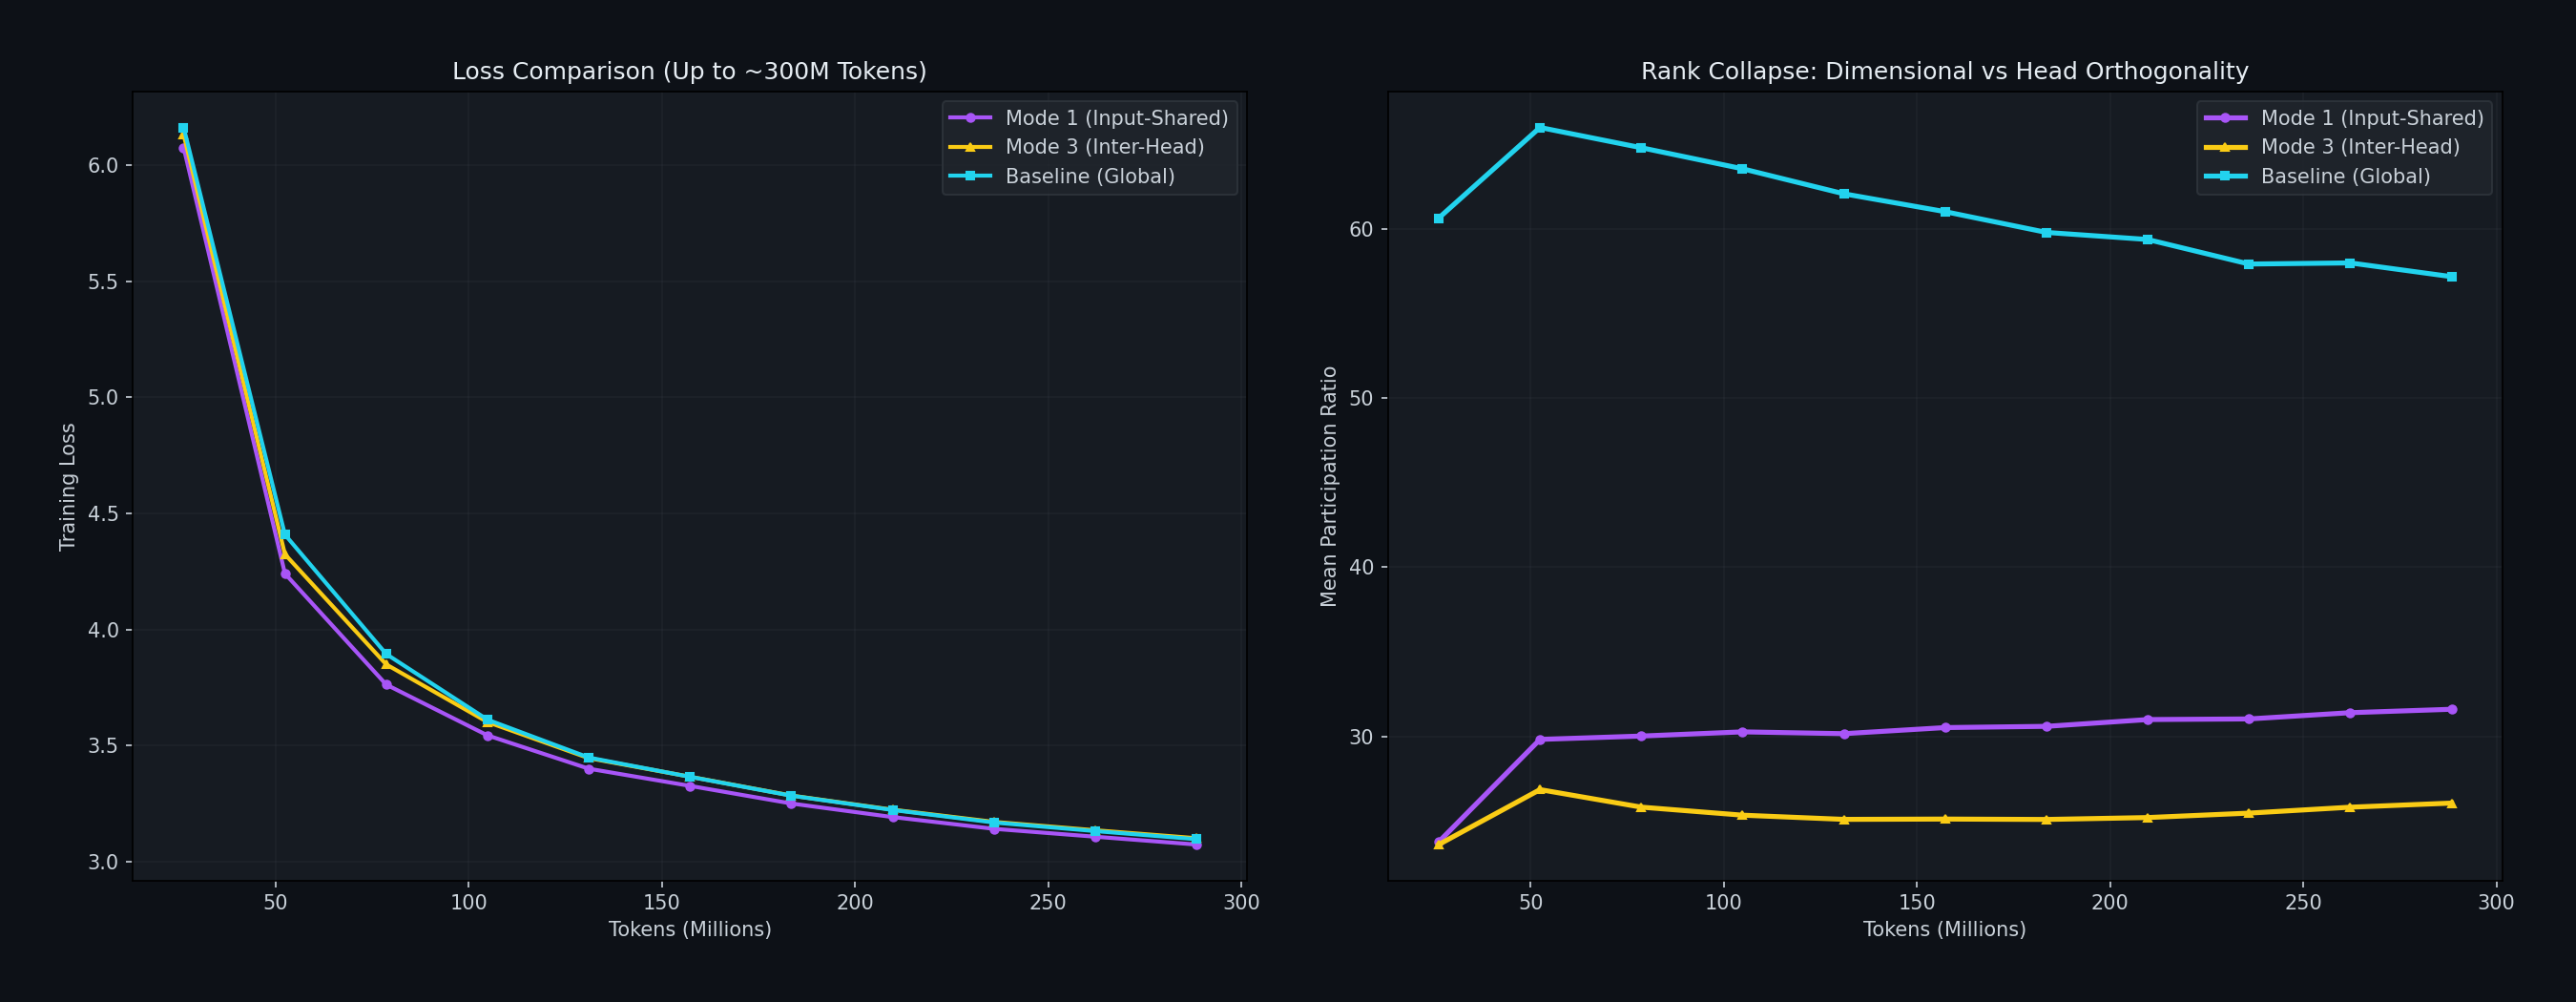
\includegraphics[width=\textwidth]{results_1b/comparison_300m_tokens.png}
\end{center}

这些结果可以用来通过最优的正交化约束 (orthogonalization constraints) 加速大语言模型 (LLM) 的预训练。

主要结论是 —— 你越是强制 LLM 的各个部分保持正交 (orthogonal)，它在早期的学习速度就越慢，但在后期的学习速度就越快。

较少的正交化会使得更多的维度坍缩 (collapse) 到接近 0 的状态，这使得损失 (loss) 在早期下降得更快，但这在训练的后期会成为一个瓶颈。

我运行了三个 LLM 训练实验，通过 Muon 优化器测试不同的正交化约束。Muon 的工作原理是强制梯度矩阵的行正交（独立）。在将梯度张量交由 Muon 处理之前，通过改变其形状 (reshaping)，我们可以重新定义什么是“行 (row)”，从而控制\textit{什么}必须独立于\textit{什么}。

我将这些约束应用于一个约 6.5 亿 (650M) 参数的 LLM 的查询和键投影（Query and Key projections，$W_Q$ 和 $W_K$）。

以下是我比较的 3 种设置：
\begin{enumerate}
    \item \textbf{标准 Muon (Baseline, 基线)}：全局正交性 (Global orthogonality)。每一个注意力头 (head) 的每一个单一维度都必须与其它所有事物独立。这强制了最大程度的多样性。
    \item \textbf{模式 1 (Input-Shared / HeadOrtho, 输入共享)}：共享子空间 (Shared subspace)。它强制第 $i$ 个特征维度独立于第 $j$ 个特征维度，但允许\textit{不同头}中具有相同索引的特征完全相同。不同的头可以自然地对齐并协作。
    \item \textbf{模式 3 (Inter-Head, 头间)}：独立头。作为整体的头 1 必须与作为整体的头 2 正交。然而，单个头\textit{内部}的特征可以完全相关。
\end{enumerate}

请在下面找到更详细的解释。

\subsection*{结果 (The Results)}

我追踪了训练损失 (Training Loss) 和参与率 (Participation Ratio, PR)，参与率是一种测量查询和键投影矩阵的“有效秩 (effective rank)”的方法。对于具有奇异值 $\sigma_i$ 的矩阵，PR 的计算公式为：
\begin{equation}
\text{PR} = \frac{(\sum \sigma_i^2)^2}{\sum \sigma_i^4}
\end{equation}
如果 PR 保持在高位，矩阵就充分利用了其多样化的容量 (许多维度都远离 0)。如果 PR 下降，意味着表示正在坍缩和变得相关 (某些维度接近 0)。

我们训练了 3 亿 (300 million) 个词元 (tokens)。\textit{（注：对于一个完整的 LLM 来说这太短了，但在我们扩大算力规模之前，它提供了强有力的初步信号）}。

\subsubsection*{3亿个词元时的定量结果 (Quantitative Results at 300M Tokens)}

\begin{table}[h]
\centering
\color{lighttext}
\begin{tabularx}{\textwidth}{l X X X}
\toprule
指标 (Metric) & \textbf{模式 1 (Input-Shared)} & \textbf{模式 3 (Inter-Head)} & \textbf{基线 (Standard Muon)} \\
\midrule
\textbf{最终训练损失 (Final Train Loss)} & \textbf{3.073} & 3.100 & 3.096 \\
\textbf{最终参与率 (Final PR)} & 31.6 & 26.1 & \textbf{57.2} \\
\bottomrule
\end{tabularx}
\end{table}

\subsection*{图表和表格告诉我们什么 (What the Graphs and Table Tell Us)}

\noindent\begin{minipage}{\linewidth}
如果我们分析上面的数据，会发现一些非常明显的（并且有些极其怪异的）行为：

\begin{center}
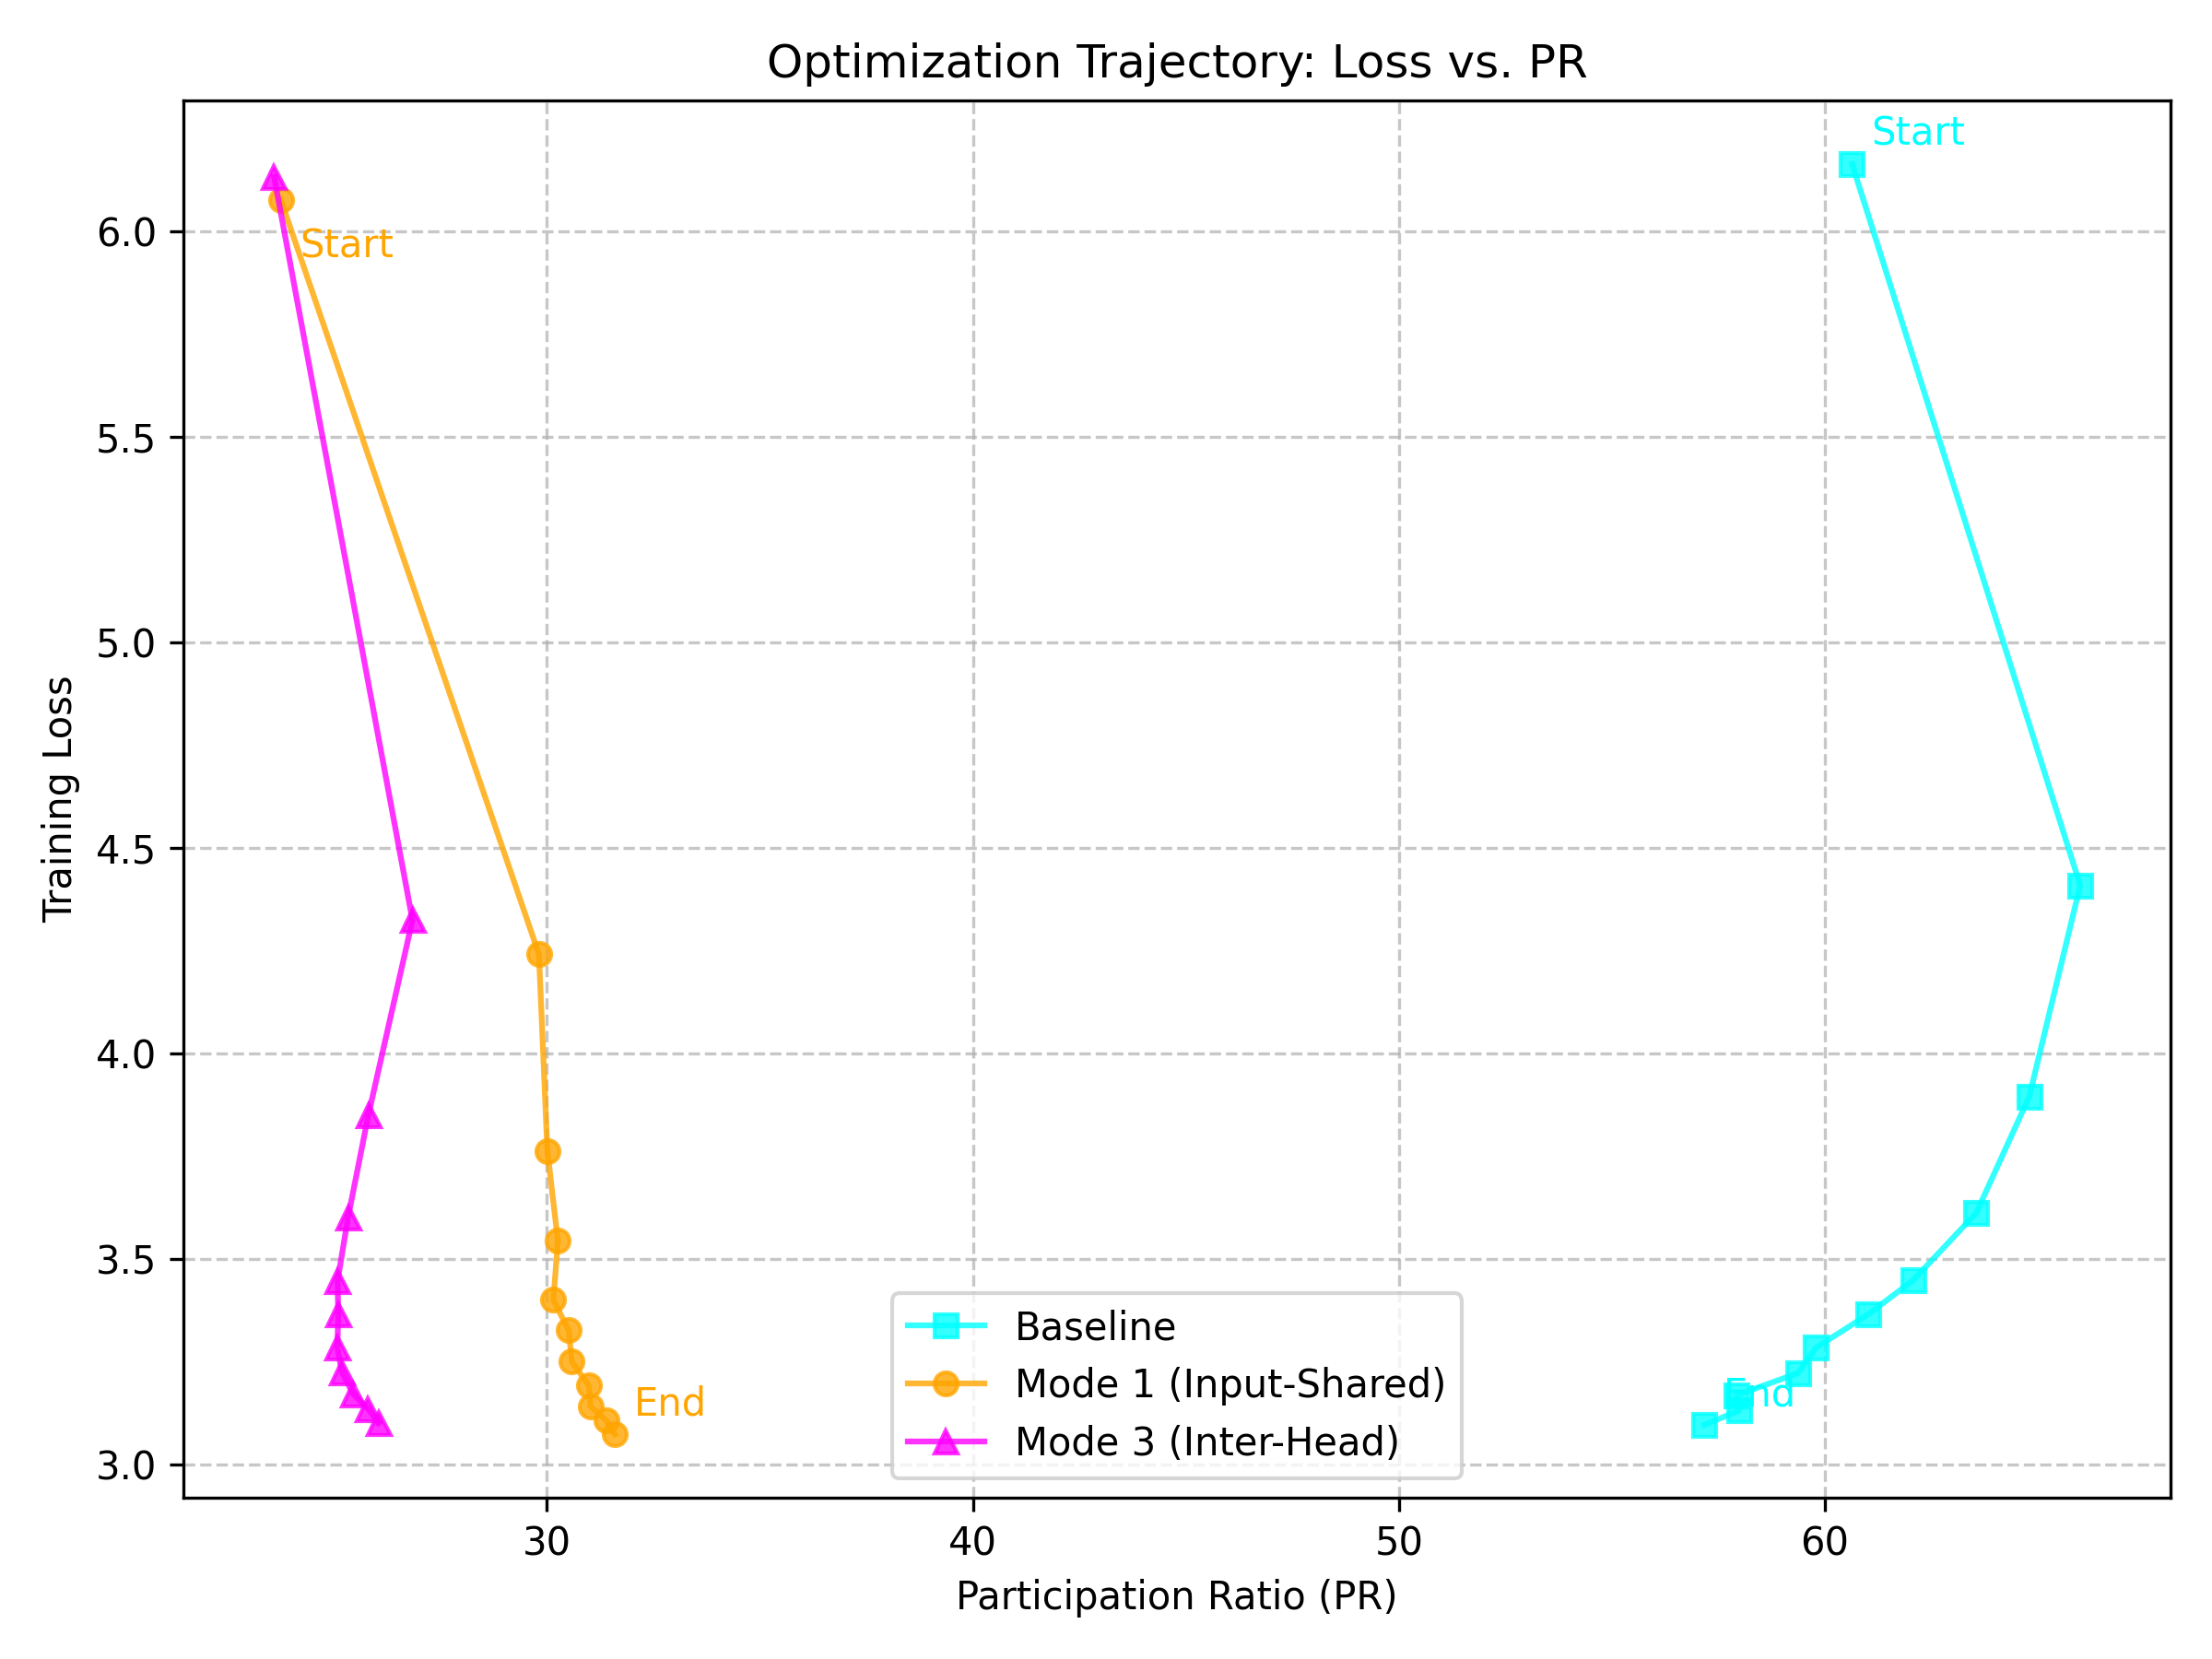
\includegraphics[width=0.9\textwidth]{results_1b/trajectory_loss_vs_pr.png}
\end{center}
\textit{这张轨迹图追踪了每种模式从开始到结束的路径。请注意，基线 (Baseline, 青色) 在损失下降的同时，其参与率 (PR) 也在缓慢流失。相比之下，模式 1 (橙色) 在早期经历了突然的秩坍缩 (rank collapse)，但随着它获得更低的整体损失，它的 PR 开始缓慢恢复并向右偏移。为了看到最终结果，需要更长时间的训练（我们目前正在处理更多的算力）。}
\end{minipage}
\vspace{1em}

\noindent\begin{minipage}{\linewidth}
\textbf{1. Muon 非常擅长保持高秩 (Forced Diversity, 强制多样性)}

\vspace{1em}
\begin{center}
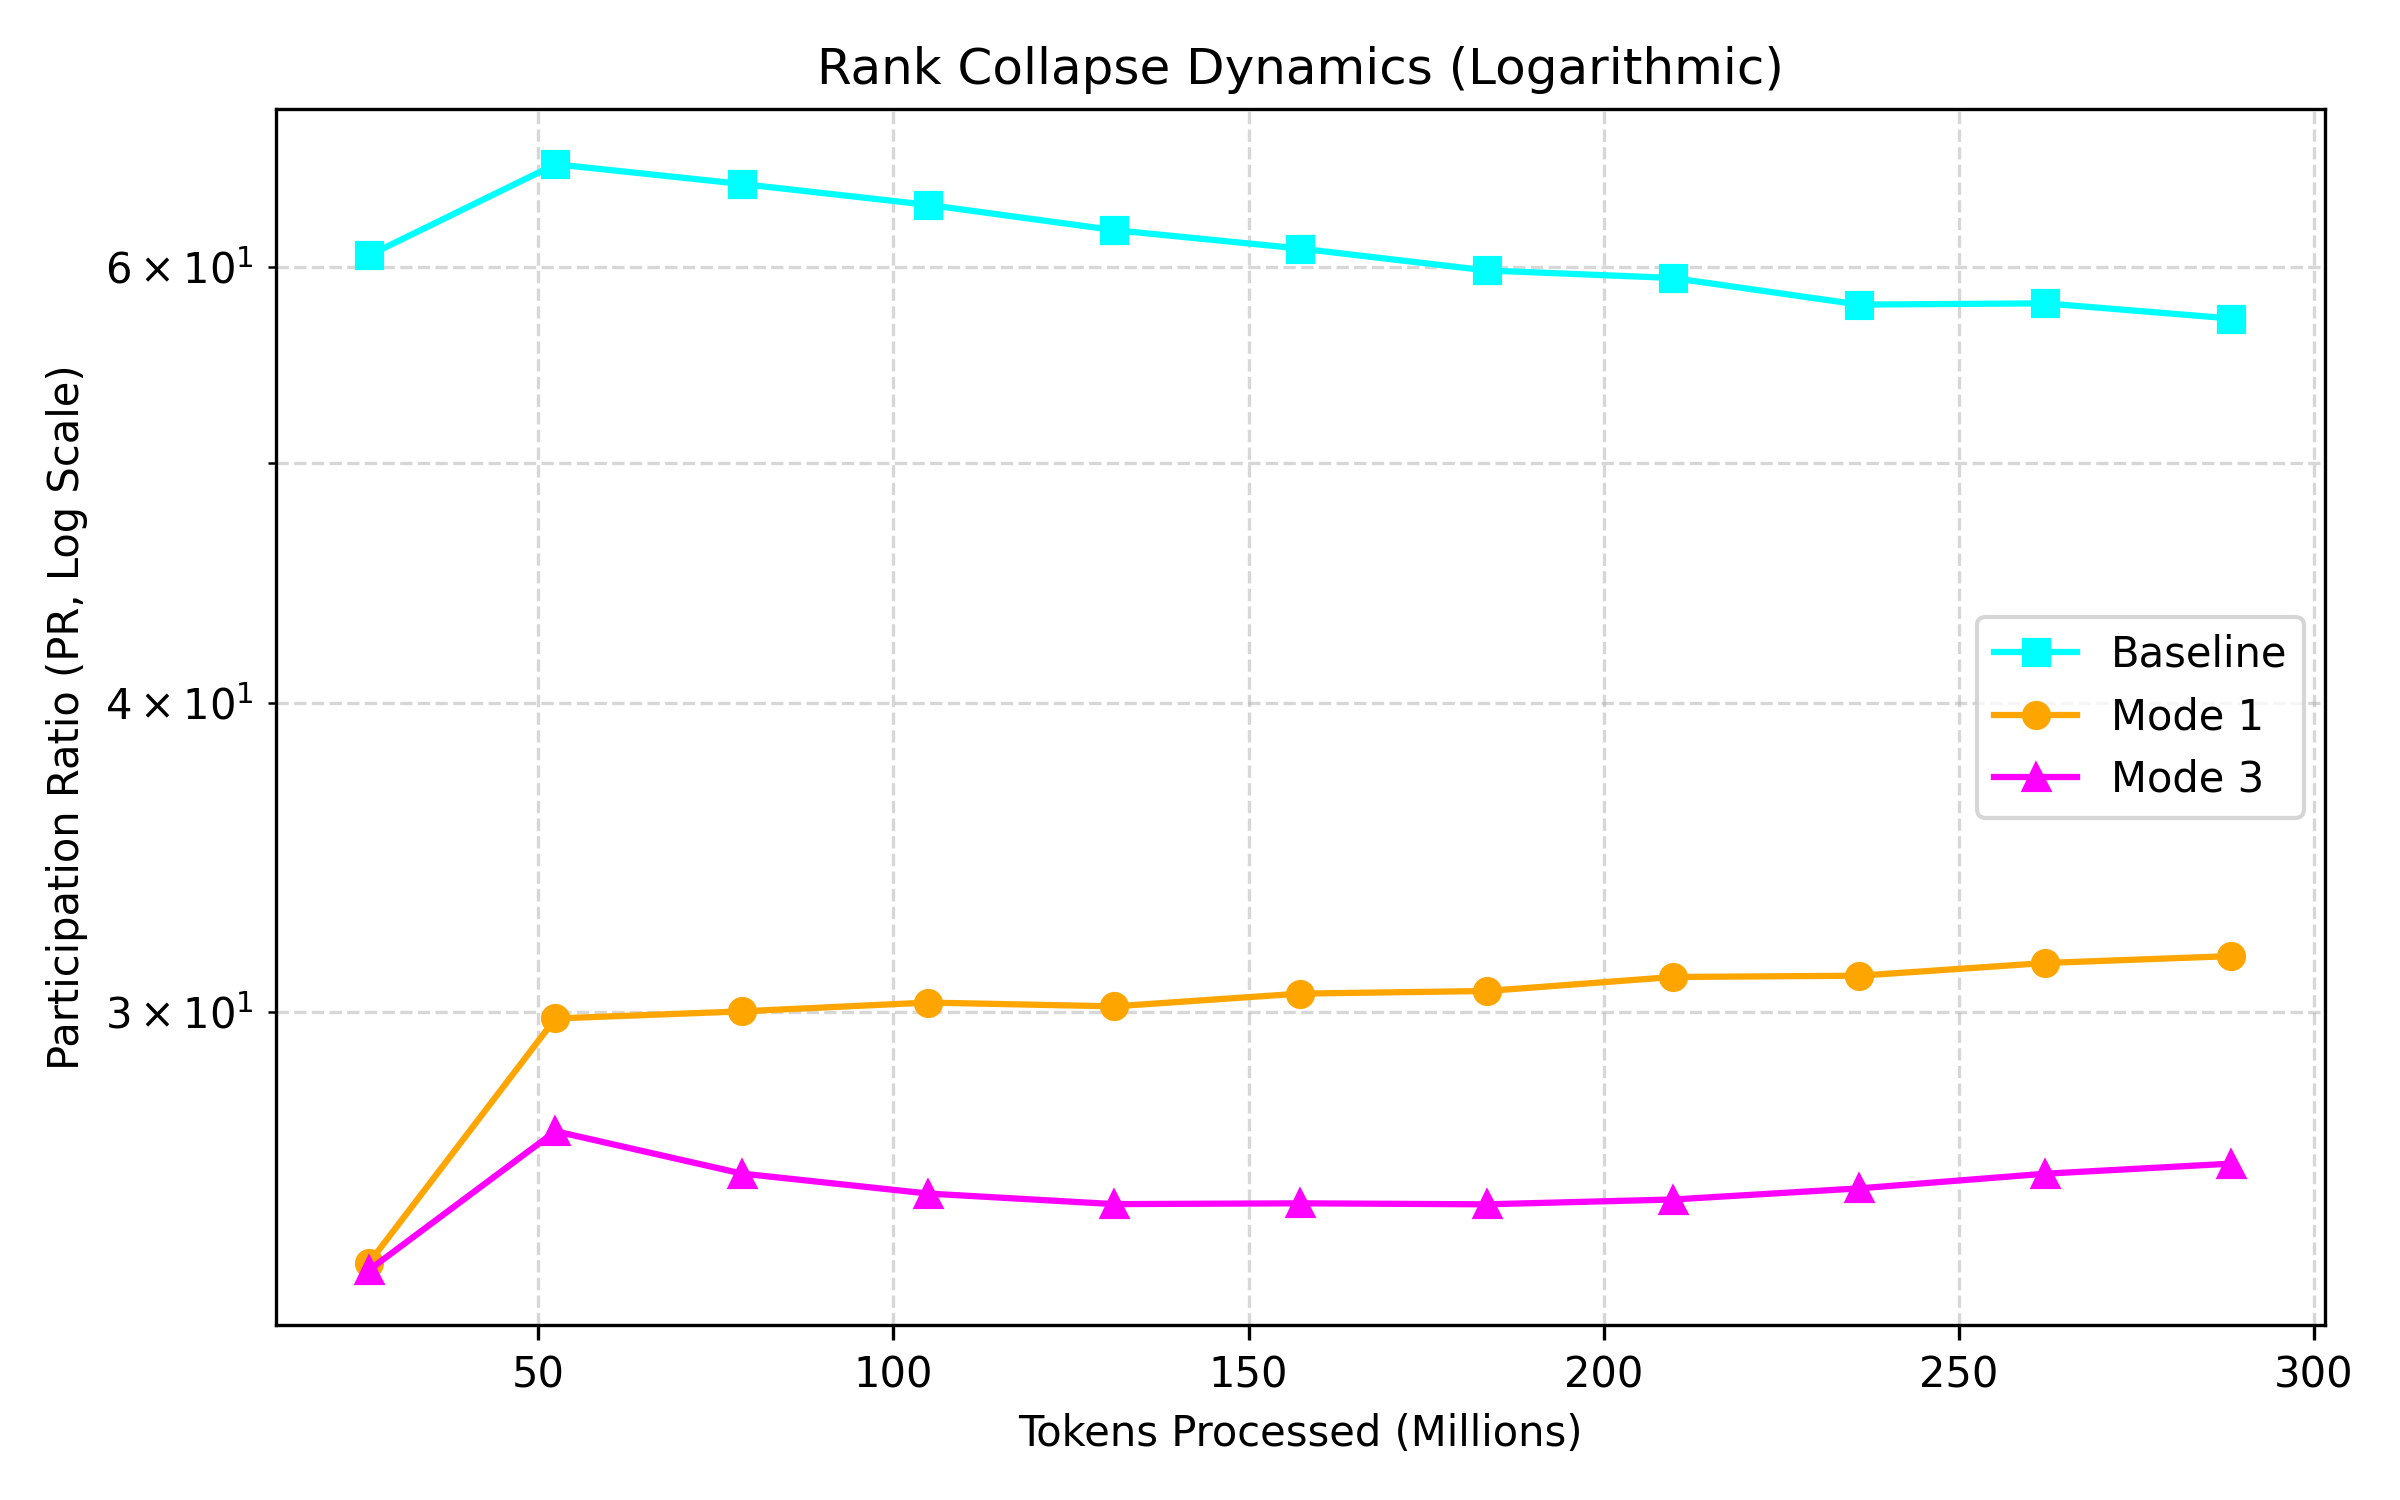
\includegraphics[width=0.9\textwidth]{results_1b/pr_log_scale.png}
\end{center}
\end{minipage}

\begin{itemize}
    \item \textbf{基线 (青色方块)} 正面对抗了模型自然简化的趋势。通过在所有部分强制执行严格的、大规模的正交性，标准 Muon 证明它非常擅长保持高参与率 ($\sim$57.2)。但是，它并没有被完美地保留下来——随着时间的推移，即使是基线也表现出缓慢的、持续的秩衰减。
    \item 相比之下，当我们放松头内部的约束时 (模式 1 和 模式 3 的正交性要求较低)，模型非常乐意在早期抛弃其多样性，并经历了大规模的秩坍缩。但在最初的崩溃之后，它们的 PR 逐渐开始缓慢攀升，并在我们训练窗口的末期积极改善。需要更多的训练才能看到那些 PR 最终会停在哪里。
\end{itemize}

\noindent\begin{minipage}{\linewidth}
\textbf{2. 坍缩的头在早期给出了更好的损失，但似乎基线正在追赶！}

\vspace{1em}
\begin{center}
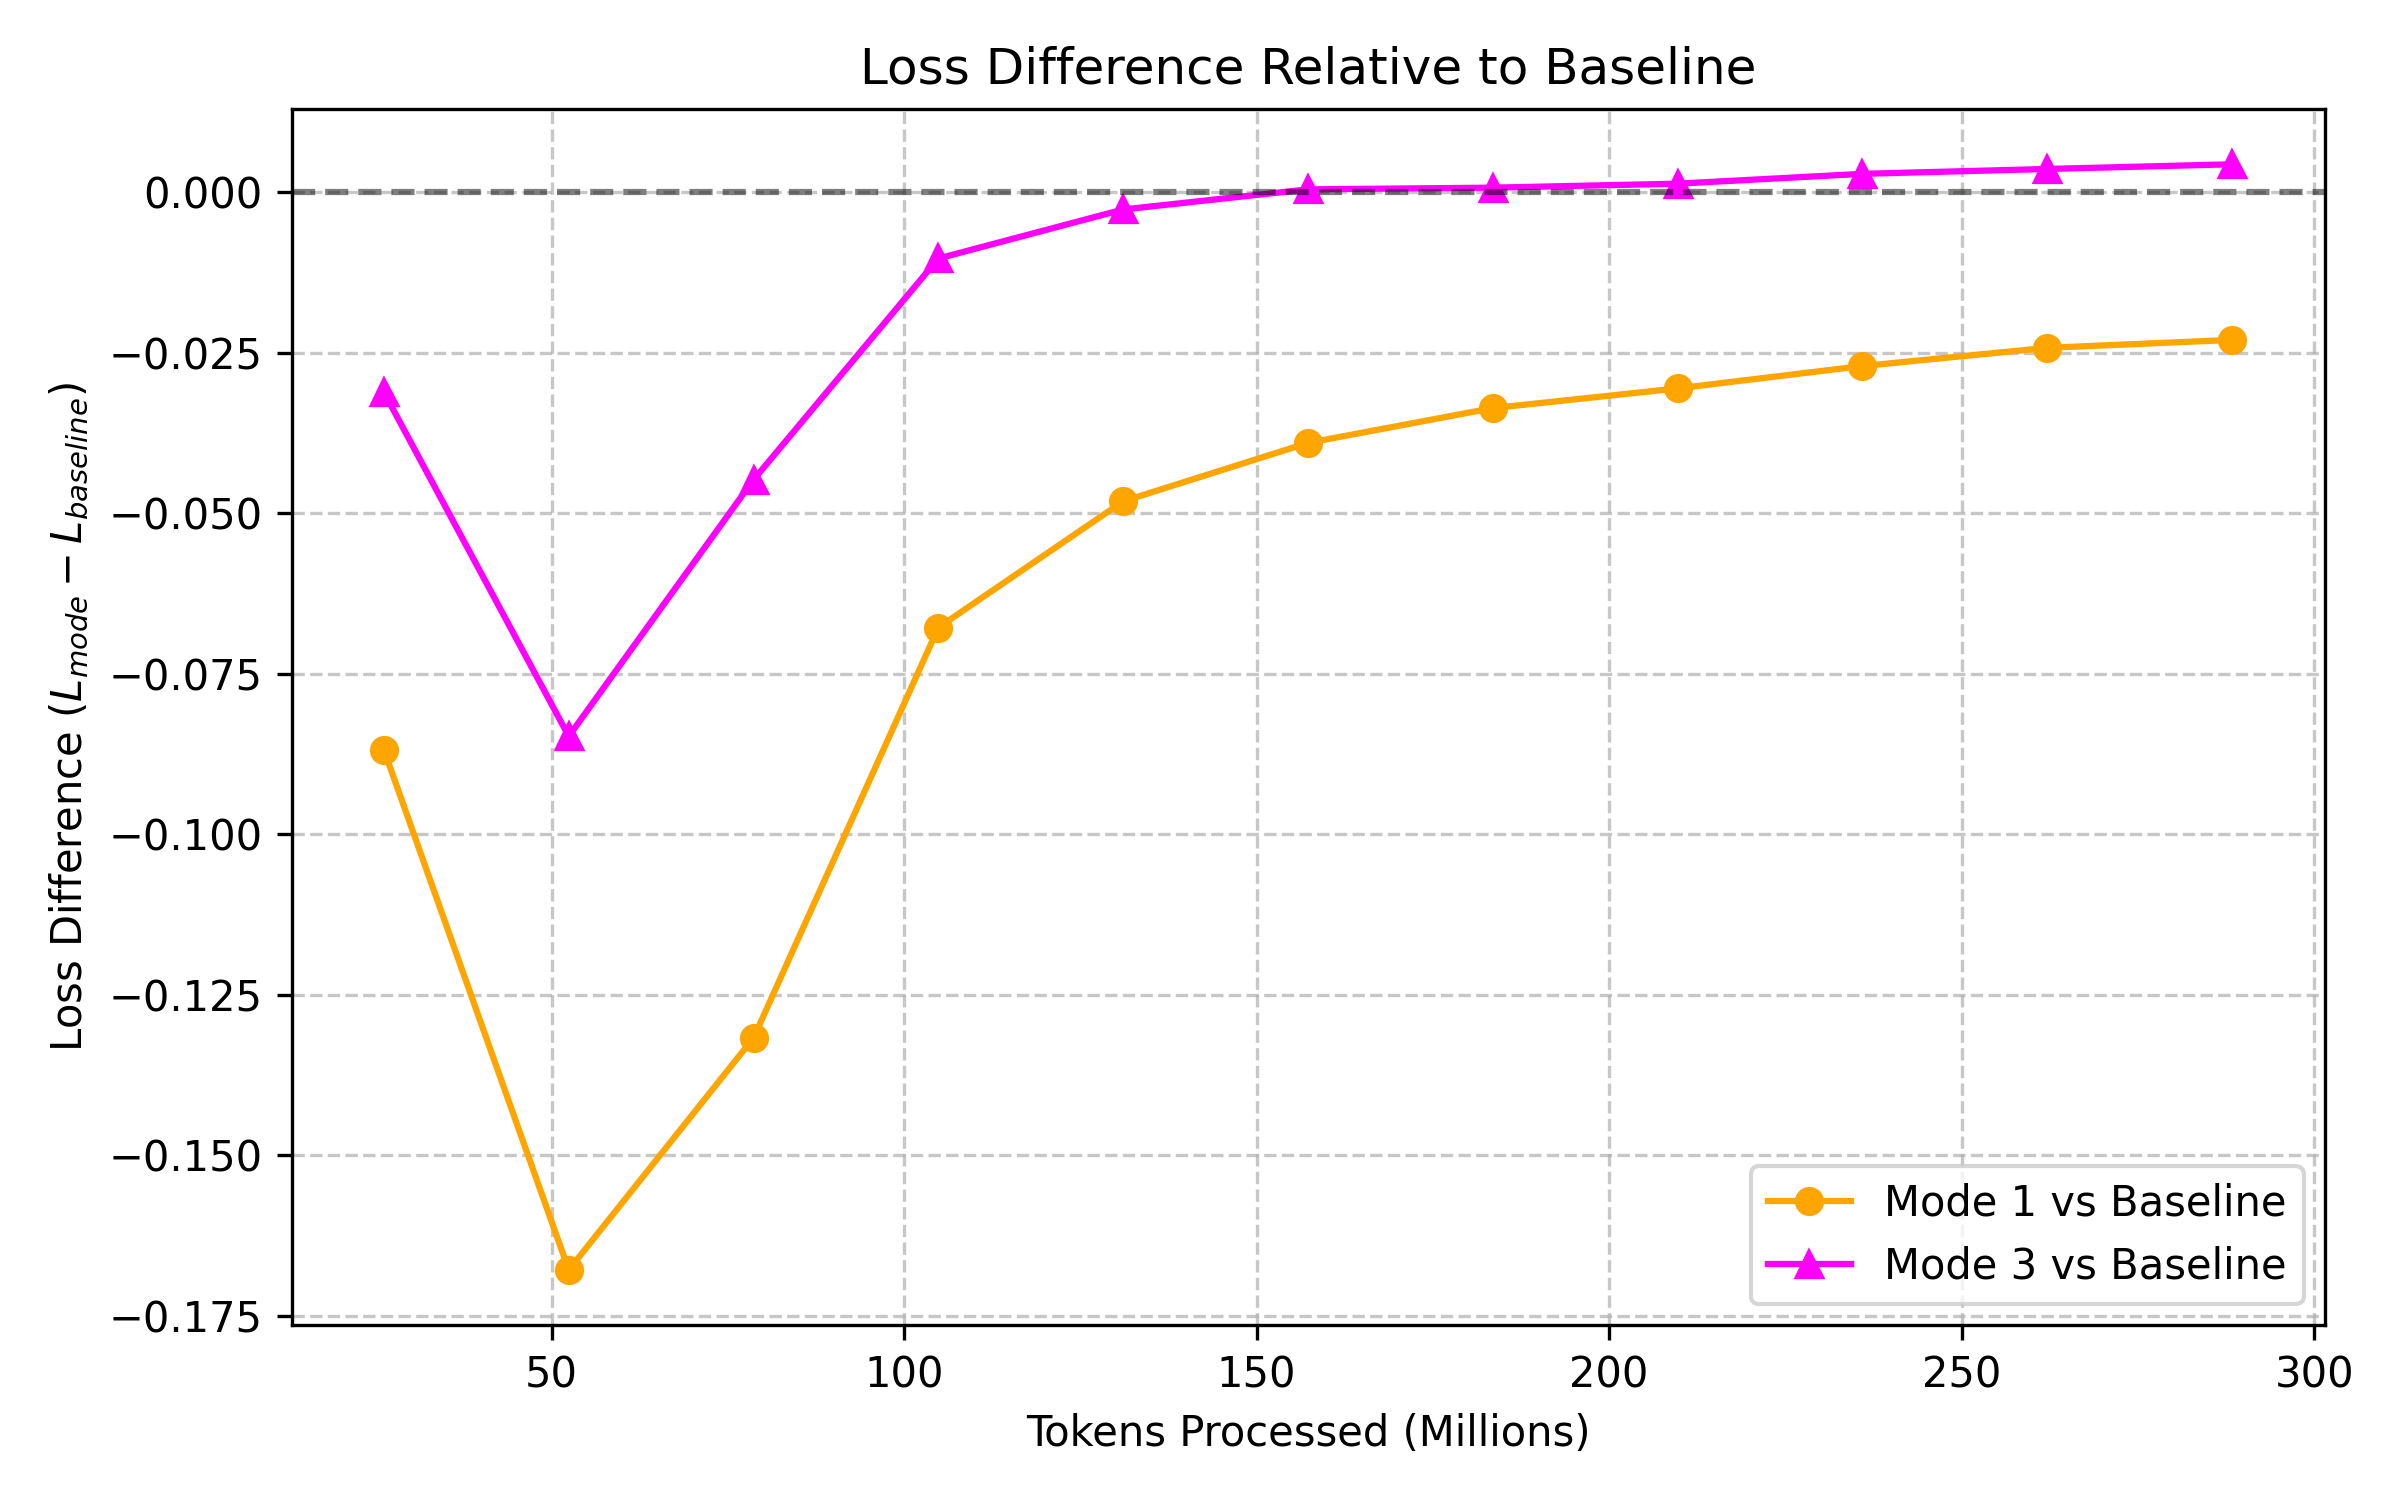
\includegraphics[width=0.9\textwidth]{results_1b/loss_difference_relative.png}
\end{center}
\end{minipage}

\begin{itemize}
    \item 尽管早期经历了大规模的秩坍缩，但\textbf{模式 1 最初下降得最快}，并且目前保持着最低的训练损失 (3.073)。
    \item 然而，虽然模式 1 取得了早期的领先优势，但基线强制执行的多样性似乎正在获得回报。模式 1 和基线之间的损失差异在 -0.16 左右达到峰值，但此后一直在缩小。
\end{itemize}

\vspace{1em}

\section*{Muon 优化中的头正交性：实验设置 (Head Orthogonality in Muon Optimization: Experimental Setup)}

\subsection*{技术细节：实验设置与方法论 (Technical Details: Experimental Setup \& Methodology)}

\textit{（本节详细介绍了总结的上述三种模式背后的数学结构）。}

为了从数学上理解这些消融实验 (ablations)，我们要看看在 Muon 固有的行正交化之前，重塑 (rearranging) 梯度张量 $G$ 是如何影响哪些参数被迫保持独立的。

\subsection*{1. 方法论：正交性的三种模式 (Methodology: Three Modes of Orthogonality)}

我们研究了牛顿-舒尔茨 (Newton-Schulz) 迭代期间梯度张量 $G$ 的形状是如何影响键/查询投影（Key/Query projections, $W_{QK} \in \mathbb{R}^{H \cdot d_k \times d_{model}}$）的学习动态的。

\subsubsection*{维度约束总结 (Summary of Dimensional Constraints)}

核心区别在于，哪些组件被强制放入相同的“行”中（并因此被迫与其他组件正交），而哪些组件则处于相同的“向量”中（从而被允许对齐）。

\begin{table}[h]
\centering
\color{lighttext}
\begin{tabularx}{\textwidth}{l X X X}
\toprule
模式 (Mode) & 重塑目标 (Reshape Target) & 正交层次 (Hierarchy of Ortho) & 有效约束 (Effective Constraint) \\
\midrule
\textbf{基线 (Baseline)} & $(H \cdot d_k) \times d_{model}$ & 一切 $\perp$ 一切 & \textbf{最强约束。} 最大化头多样性。 \\
\textbf{模式 1 (Mode 1)} & $d_k \times (H \cdot d_{model})$ & 行索引 $\perp$ 行索引 & \textbf{共享子空间。} 头被水平拼接。 \\
\textbf{模式 3 (Mode 3)} & $H \times (d_k \cdot d_{model})$ & 头 $\perp$ 头 & \textbf{独立头。} 内部行可对齐。 \\
\bottomrule
\end{tabularx}
\end{table}

\begin{itemize}
    \item \textbf{基线} 指示：“每一个单独的头部的权重投影矩阵的每一行 (参数向量) 都必须是唯一的，并且与所有其他行正交。”
    \item \textbf{模式 1} 指示：“头 1 的第 $i$ 行和头 2 的第 $i$ 行属于同一长向量。它们必须垂直于任何第 $j$ 行 ($i \neq j$)，但头 1 和头 2 可以在第 $i$ 维度上使用相同的权重。”
    \item \textbf{模式 3} 指示：“头 1 必须作为一个整体（其所有行相结合）正交于头 2 (作为一个整体)。与基线不同，它并不关心头 1 \textit{内部} 的行是否相似，只要 ‘头 1 子空间’ 正交于 ‘头 2 子空间’ 即可。”
\end{itemize}

\subsubsection*{1.1 基线：全局矩阵正交性 (Baseline: Global Matrix Orthogonality)}
\textbf{标准 Muon (Standard Muon)} 将整个参数矩阵视为一个单独的 2D 张量。
$$G_{\text{base}} \in \mathbb{R}^{(H \cdot d_k) \times d_{model}}$$
其中：
\begin{itemize}
    \item $H$ 是注意力头的数量（例如：16）。
    \item $d_k$ 是每个头的维度（例如：128）。
    \item $d_{model}$ 是输入的隐藏层维度（例如：2048）。
    \item \textbf{每个元素 $W_{QK}^{h,i}$ 代表头 $h$ 的 QK 投影矩阵的第 $i$ 个行向量。}其大小为 $d_{model}$。
\end{itemize}

优化器使这一个巨大矩阵的行正交化。
\begin{itemize}
    \item \textbf{约束}：每一行（每一个头的一个维度）都要与组合矩阵中的其他所有行进行正交化。
    \item \textbf{效果}：这强制要求所有 $H \cdot d_k$ 个输出维度同时存在一个整体的多样性约束。
\end{itemize}

\textbf{示例 ($H=2, d_k=2$)：}
所有事物必须与其他所有事物正交。每行是一个大小为 $d_{model}$ 的权重向量。

\begin{table}[h]
\centering
\color{lighttext}
\begin{tabularx}{\textwidth}{l X X X}
\toprule
矩阵行 (Matrix Row) & 代表的权重向量 (Weight Vec) & 正交于 (Orthogonal to:) & 含义 (Meaning) \\
\midrule
行 1 & $W_{QK}^{1,1}$ & 行 2, 3, 4 & $W_{QK}^{1,1} \neq W_{QK}^{1,2}, W_{QK}^{2,1}$ 等 \\
\textbf{行 2} & $W_{QK}^{1,2}$ & 行 1, 3, 4 & 头 1 内部的特征正交。 \\
\textbf{行 3} & $W_{QK}^{2,1}$ & 行 1, 2, 4 & 头 2 正交于头 1。 \\
\textbf{行 4} & $W_{QK}^{2,2}$ & 行 1, 2, 3 & 头 2 内部的特征正交。 \\
\bottomrule
\end{tabularx}
\end{table}

\textbf{可视矩阵 (Visual Matrix) ($4 \times d_{model}$)：}
$$
G_{\text{base}} = 
\begin{bmatrix}
w_{1,1,1} & w_{1,1,2} & \dots & w_{1,1,D} \\
w_{1,2,1} & w_{1,2,2} & \dots & w_{1,2,D} \\
w_{2,1,1} & w_{2,1,2} & \dots & w_{2,1,D} \\
w_{2,2,1} & w_{2,2,2} & \dots & w_{2,2,D}
\end{bmatrix}
\begin{matrix}
\leftarrow W_{QK}^{1,1} \text{ (头 1, 行 1)} \\
\leftarrow W_{QK}^{1,2} \text{ (头 1, 行 2)} \\
\leftarrow W_{QK}^{2,1} \text{ (头 2, 行 1)} \\
\leftarrow W_{QK}^{2,2} \text{ (头 2, 行 2)}
\end{matrix}
$$
所有 4 行都会彼此正交化。

\subsubsection*{1.2 模式 1：输入共享的正交性 (Mode 1: Input-Shared Orthogonality (``HeadOrtho''))}
我们重塑梯度，以将“头维度 (head dimension)”与“特征维度 (feature dimension)”分离开，并将共享输入空间上的 $d_k$ 个特征维度正交化。
$$G_{\text{mode1}} \in \mathbb{R}^{d_k \times (H \cdot d_{model})}$$
\begin{itemize}
    \item \textbf{约束}：第 $i$ 个特征维度与第 $j$ 个特征维度正交化，该向量是聚合了所有头获得的。
    \item \textbf{结构}：这将 $H$ 个头视为在构成一个共享的 $d_k$ 维子空间。在这相同的特征维度上，并不强制不同头\textit{之间}正交。
\end{itemize}

\textbf{示例 ($H=2, d_k=2$)：}
我们只重塑为 2 个大行 ($d_k=2$)。每一行是所有头中该特征行的\textit{拼接 (concatenation)}。

\begin{table}[h]
\centering
\color{lighttext}
\begin{tabularx}{\textwidth}{l X X X}
\toprule
矩阵行 (Matrix Row) & 代表的拼接向量 (Concat Vec) & 正交于 (Orthogonal to:) & 含义 (Meaning) \\
\midrule
\textbf{行 1} & $W_{QK}^{1,1} \oplus W_{QK}^{2,1}$ & 行 2 & 行 1 子空间 $\perp$ 行 2 子空间。 \\
\textbf{行 2} & $W_{QK}^{1,2} \oplus W_{QK}^{2,2}$ & 行 1 & \textbf{$W_{QK}^{1,1}$ 和 $W_{QK}^{2,1}$ 可以完全相同。} \\
\bottomrule
\end{tabularx}
\end{table}

\textbf{可视矩阵 (Visual Matrix) ($2 \times 2 \cdot d_{model}$)：}
$$
G_{\text{mode1}} = 
\begin{bmatrix}
\underbrace{w_{1,1,1} \dots w_{1,1,D}}_{W_{QK}^{1,1} \text{ (头 1)}} & \mathbf{|} & \underbrace{w_{2,1,1} \dots w_{2,1,D}}_{W_{QK}^{2,1} \text{ (头 2)}} \\
\underbrace{w_{1,2,1} \dots w_{1,2,D}}_{W_{QK}^{1,2} \text{ (头 1)}} & \mathbf{|} & \underbrace{w_{2,2,1} \dots w_{2,2,D}}_{W_{QK}^{2,2} \text{ (头 2)}}
\end{bmatrix}
$$
只有顶行 $\perp$ 底行。 头 1 和头 2 仅仅是同一行向量中的不同列部分！

\subsubsection*{1.3 模式 3：头间正交性 (Mode 3: Inter-Head Orthogonality)}
我们重塑梯度以迫使各个头彼此正交。
$$G_{\text{mode3}} \in \mathbb{R}^{H \times (d_k \cdot d_{model})}$$
\begin{itemize}
    \item \textbf{约束}：\texttt{头 i} 的梯度更新向量会与 \texttt{头 j} 进行正交化。
    \item \textbf{结构}：这专门针对注意力头的独立性，将每个头视为参数空间中的一个单位向量。
\end{itemize}

\textbf{示例 ($H=2, d_k=2$)：}
我们重塑为只有 2 个大行（每个头有一个，所以 $H=2$）。 每一行是该头内所有特征行的\textit{拼接 (concatenation)}。

\begin{table}[h]
\centering
\color{lighttext}
\begin{tabularx}{\textwidth}{l X X X}
\toprule
矩阵行 (Matrix Row) & 代表的拼接向量 (Concat Vec) & 正交于 (Orthogonal to:) & 含义 (Meaning) \\
\midrule
\textbf{行 1} & $W_{QK}^{1,1} \oplus W_{QK}^{1,2}$ & 行 2 & \textbf{头 1 必须正交于头 2。} \\
\textbf{行 2} & $W_{QK}^{2,1} \oplus W_{QK}^{2,2}$ & 行 1 & 头内特征可以是任何组合 (只要 $\perp$ H1)。 \\
\bottomrule
\end{tabularx}
\end{table}

\textbf{可视矩阵 (Visual Matrix) ($2 \times 2 \cdot d_{model}$)：}
$$
G_{\text{mode3}} = 
\begin{bmatrix}
\underbrace{w_{1,1,1} \dots w_{1,1,D}}_{W_{QK}^{1,1}} & \mathbf{|} & \underbrace{w_{1,2,1} \dots w_{1,2,D}}_{W_{QK}^{1,2}} \\
\underbrace{w_{2,1,1} \dots w_{2,1,D}}_{W_{QK}^{2,1}} & \mathbf{|} & \underbrace{w_{2,2,1} \dots w_{2,2,D}}_{W_{QK}^{2,2}}
\end{bmatrix}
\begin{matrix}
\leftarrow \text{头 1 参数 (Head 1 Parameters)} \\
\leftarrow \text{头 2 参数 (Head 2 Parameters)}
\end{matrix}
$$
顶行 (头 1) $\perp$ 底行 (头 2)。

\vspace{1em}

\subsection*{2. 实验设置 (Experimental Setup)}

为了比较这些模式，我们训练了一个约 6.5 亿参数的语言模型。

\subsubsection*{2.1 模型架构 (Model Architecture)}
\begin{itemize}
    \item \textbf{参数量 (Parameters)}：约 6.5 亿 (650 Million)
    \item \textbf{层数 (Layers)}：12
    \item \textbf{隐藏层维度 ($d_{model}$)}：2048
    \item \textbf{注意力头 (Attention Heads)}：16 (使用分组查询注意力，含 8 个 KV 头)
    \item \textbf{头维度 ($d_k$)}：128
    \item \textbf{序列长度 (Sequence Length)}：2048
\end{itemize}

\subsubsection*{2.2 训练配置 (Training Configuration)}
\begin{itemize}
    \item \textbf{数据集 (Dataset)}：SmolLM-corpus。
    \item \textbf{训练词元 (Tokens Trained)}：3 亿 (300 Million)。
    \item \textbf{批次大小 (Batch Size)}：32，梯度累积步数为 4 (等效批次大小约为 26 万 (262k) 个词元)。
    \item \textbf{优化器 (Optimizer)}：Muon (用于 2D 参数) + AdamW (用于嵌入/归一化参数)。
    \item \textbf{学习率 (Learning Rate)}：Muon LR 0.05，AdamW LR 0.005。
\end{itemize}

\subsubsection*{2.3 追踪的指标 (Metrics Tracked)}
在整个训练过程中，我们主要监测两个指标：
\begin{enumerate}
    \item \textbf{训练损失 (Training Loss)}：用于衡量优化的效率。
    \item \textbf{参与率 (Participation Ratio, PR)}：估计键/查询投影矩阵的有效秩，以量化“秩坍缩 (Rank Collapse)”与严格正交性。
\end{enumerate}

\subsection*{3. 结论 (Conclusion)}

正如本文件第一部分进行了大量绘图并讨论的那样，全局强制正交性（基线）人为地维持了投影矩阵的秩，使得在训练开始时的优化暂时变慢。放宽这个约束从而允许自然产生相关性和结构性分组（模式 1 和模式 3），会导致秩的大幅下降，但在最初带来了极快损失下降。然而，因为基线一旦开始利用其保留的多样性就会赶上进度，所以长期来看，真实的最优归纳偏置（inductive bias）仍是一个悬而未决的问题。

\end{document}
